\begin{frame}{Early Stopping}
\begin{figure}[H]
	\centering
	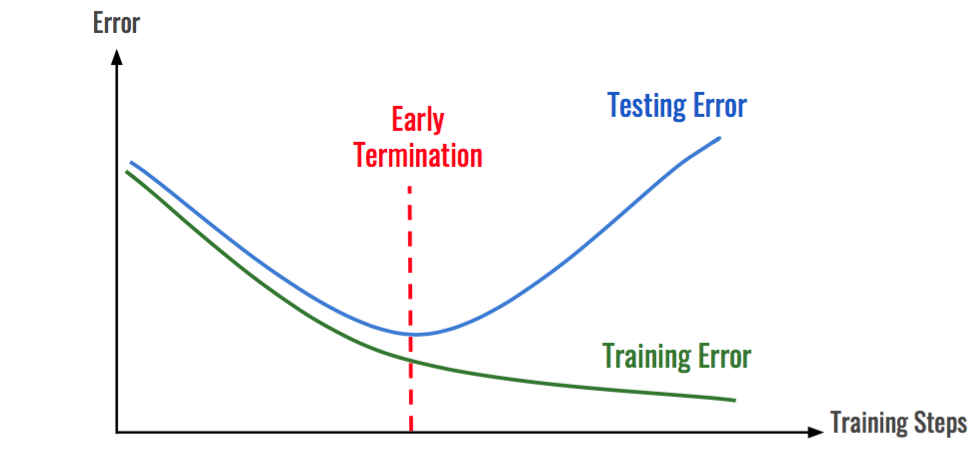
\includegraphics[width=0.6\textwidth]{Images/Early Stopping.png}
	\caption{Early Stopping. \href{https://medium.com/analytics-vidhya/early-stopping-with-pytorch-to-restrain-your-model-from-overfitting-dce6de4081c5}{Source}}
	\label{fig:Early Stopping}
\end{figure}
\begin{itemize}
\item Stop training when accuracy on the validation set decreases (or loss increases). Or keep track of the model parameters that worked best on validation set.
\end{itemize}
\end{frame}


\begin{frame}{Regularization: Add term to loss}
\begin{equation*}
\mathlarger{\mathlarger{L = \frac{1}{N} \sum_{i=1}^{N} L(\phi(x_i), y_i) + \lambda R(W)}}
\end{equation*}
\vspace{20pt}


Common regularization terms:
%\begin{tabular}{l@{\hspace{0.3\textwidth}}l}
%L2 regularization & $R(W)=\sum_{k}\sum_l W_{k,l}^2$\\
%L1 regularization & $R(W)=\sum_{k}\sum_l W_{k,l}^2$\\
%Elastic net (L1 + L2) & $R(W)=\sum_{k}\sum_l \beta W_{k,l}^2 + \vert W_{k,l}^2\vert$\\
%\end{tabular}
\begin{columns}
\begin{column}{0.5 \textwidth}
\begin{itemize}
\item L2 regularization
\item L1 regularization
\item Elastic net (L1 + L2)
\end{itemize}
\end{column}
\begin{column}{0.5 \textwidth}
$R(W)=\sum_{k}\sum_l W_{k,l}^2$ \\
$R(W)=\sum_{k}\sum_l W_{k,l}^2$\\
$R(W)=\sum_{k}\sum_l \beta W_{k,l}^2 + \vert W_{k,l}^2\vert$\\
\end{column}
\end{columns}
\end{frame}

\begin{frame}{Regularization: Dropout}
\begin{itemize}
	\item Randomly set some of neurons to zero in forward pass.
\end{itemize}
\begin{figure}[H]
\centering
\begin{subfigure}[b]{0.3\textwidth}
	\centering
	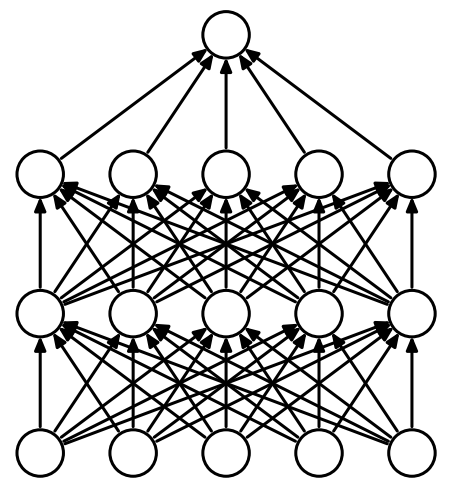
\includegraphics[width=\textwidth]{Images/Dropout-before.png}
	\caption{Without using dropout}
	\label{fig:Dropout-before}
\end{subfigure}
\begin{subfigure}[b]{0.3\textwidth}
	\centering
	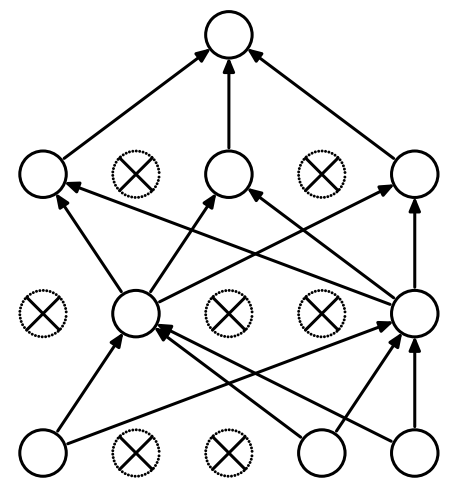
\includegraphics[width=\textwidth]{Images/Dropout-after.png}
	\caption{After using dropout.}
	\label{fig:Dropout-after}
\end{subfigure}
\caption{Behavior of dropout at training time. \href{https://www.cs.toronto.edu/~hinton/absps/JMLRdropout.pdf}{Source}}
\end{figure}
\end{frame}

\begin{frame}{Regularization: Dropout}
\noindent\begin{minipage}{0.4\textwidth}
\begin{figure}[H]
	\centering
	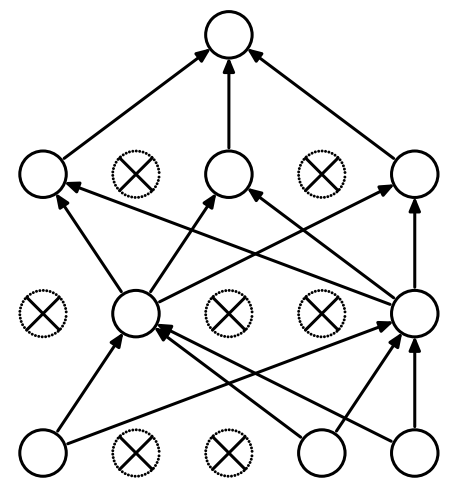
\includegraphics[width=\textwidth]{Images/Dropout-after.png}
	\caption{\href{https://www.cs.toronto.edu/~hinton/absps/JMLRdropout.pdf}{Source}}
\end{figure}
\end{minipage}
\noindent\begin{minipage}{0.4\textwidth}
\begin{itemize}
	\item Dropout:
	\begin{itemize}
		\item Prevents co-adaptation of features (forces network to have redundant representations).
		\item Can be considered a large ensemble of models sharing parameters.
	\end{itemize}
\end{itemize}
\end{minipage}
\end{frame}

\begin{frame}{Dropout: Test Time}
\begin{itemize}
\item Dropout makes output of network random!
\begin{center}
\begin{tabular}{l@{\hspace{0.25\textwidth}}l}
&$z$: random mask\\
$y = f_W(x, z)$
& $x$: input of the layer\\
& $y$: output of the layer\\
\end{tabular}
\end{center}
\item We want to "average out" the randomness at test time:
\begin{equation*}
y=f(x)=\mathbb{E}_z[f(x, z)] = \sum_z p(z)f(x, z)dz
\end{equation*}

\item Can we calculate the integral exactly?\\
\pause
\item We need to approximate the integral.
\end{itemize}
\end{frame}

\begin{frame}{Dropout: Test Time}
\begin{itemize}
	\item Consider a simple case:
\end{itemize}
\begin{columns}
\begin{column}{0.4 \textwidth}
\begin{center}
	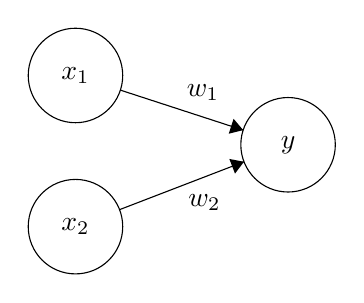
\begin{tikzpicture}[scale=0.2]
		\tikzstyle{every node}+=[inner sep=0pt]
		\draw [black] (37.4,-25.4) circle (3);
		\draw (37.4,-25.4) node {$y$};
		\draw [black] (23.9,-21) circle (3);
		\draw (23.9,-21) node {$x_1$};
		\draw [black] (23.9,-30.6) circle (3);
		\draw (23.9,-30.6) node {$x_2$};
		\draw [black] (26.75,-21.93) -- (34.55,-24.47);
		\fill [black] (34.55,-24.47) -- (33.94,-23.75) -- (33.63,-24.7);
		\draw (31.99,-22.64) node [above] {$w_1$};
		\draw [black] (26.7,-29.52) -- (34.6,-26.48);
		\fill [black] (34.6,-26.48) -- (33.67,-26.3) -- (34.03,-27.23);
		\draw (32.09,-28.53) node [below] {$w_2$};
	\end{tikzpicture}
\end{center}

\end{column}
\begin{column}{0.6 \textwidth}
\begin{itemize}
\item At training time, each neuron is alive with probability of $p=0.5$:
\begin{align*}
\mathbb{E}[y] =& \frac{1}{4}(w_1x_1 + w_2x_2) + \frac{1}{4}(w_1x_1 + 0)\\
&+ \frac{1}{4}(0 + w_2x_2) + \frac{1}{4}(0 + 0)\\
=& \frac{1}{2}(w_1x_1 + w_2x_2)
\end{align*}
\item At test time:
\begin{itemize}
	\item \tc{keywords}{Multiply} by dropout rate.
\end{itemize}
\end{itemize}
\end{column}
\end{columns}
\end{frame}

\begin{frame}{Dropout: Test Time}
\begin{itemize}
	\item At test time neurons are always present and its output is multiplied by dropout probability:
\end{itemize}
\begin{figure}[H]
	\centering
	\begin{subfigure}[b]{0.3\textwidth}
		\centering
		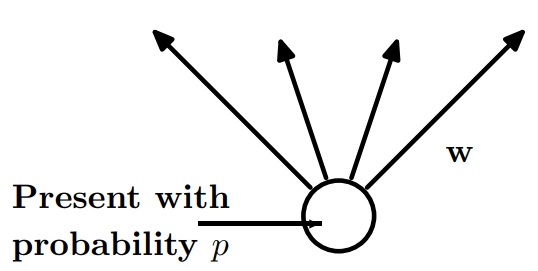
\includegraphics[width=\textwidth]{Images/dropout-test time-before.png}
		\caption{Without using dropout}
		\label{fig:dropout-test time-before}
	\end{subfigure}
	\begin{subfigure}[b]{0.3\textwidth}
		\centering
		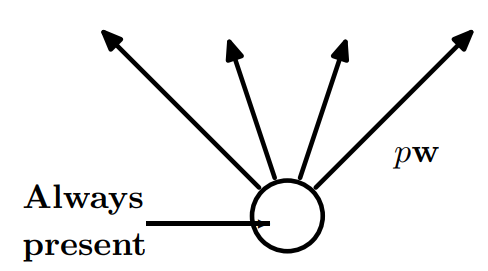
\includegraphics[width=\textwidth]{Images/dropout-test time-after.png}
		\caption{After using dropout.}
		\label{fig:dropout-test time-after}
	\end{subfigure}
	\caption{Behavior of dropout at test time. \href{https://www.cs.toronto.edu/~hinton/absps/JMLRdropout.pdf}{Source}}
\end{figure}
\end{frame}


%\begin{frame}{Regularization: Adding Noise}
%\begin{itemize}
%\item We've seen a common approach for regularization thus far:
%\begin{itemize}
%	\item \textbf{Training}: Add some kind of randomness ($z$) : $$y = f_W(x, z)$$
%	\item \textbf{Testing}: Average out the randomness: $$y=f(x)=\mathbb{E}_z[f(x, z)] = \sum_z p(z)f(x, z)dz$$
%\end{itemize}
%\pause
%\item Adding noise is another way to prevent a neural network from overfitting on the training data.
%In every iteration, a random noise is added to the outputs of the layer, preventing consequent layers from co-adapting too much to the outputs of this layer.
%\end{itemize}
%\end{frame}

\begin{frame}{Batch Normalization}
	\begin{multicols}{2}
		\begin{itemize}
			\item Input: $\pmb{x}: N\times D$
			\item Output: $\pmb{y}: N\times D$
			\item Learnable Parameters: $\pmb{\gamma}, \pmb{\beta}: 1\times D$
			\item Intermediates: $\pmb{\mu}_B, \pmb{\mu}, \pmb{\sigma}_B^2, \pmb{\sigma}^2: 1\times D$
			\item Intermediates:  $\hat{\pmb{x}}: N \times D$
			\item Hyper-parameters: m (momentum)
		\end{itemize}
	\end{multicols}
\end{frame}

\begin{frame}{Batch Normalization: Training Time}
%\begin{tabular}{l l}
%Input: $x: N\times D$ & Learnable Parameters: $\gamma, \beta: D$\\
%Output: $y: N\times D$ & Intermediates: $\mu, \sigma: D$, $\hat{x}: N \times D$
%\end{tabular}
%\begin{columns}
%\begin{column}{0.3 \textwidth}
%
%\end{column}
%\end{columns}
\begin{multicols}{2}
\begin{itemize}
\item Input: $\pmb{x}: N\times D$
\item Output: $\pmb{y}: N\times D$
\item Learnable Parameters: $\pmb{\gamma}, \pmb{\beta}: 1\times D$
\item Intermediates: $\pmb{\mu}_B, \pmb{\mu}, \pmb{\sigma}_B^2, \pmb{\sigma}^2: 1\times D$
\item Intermediates:  $\hat{\pmb{x}}: N \times D$
\item Hyper-parameters: m (momentum)
\end{itemize}
\end{multicols}

\vspace{-30pt}

\begin{align*}
\pmb{\mu}_B &= \frac{1}{N_B}\sum_{i=1}^{N_B} \pmb{x}^{(i)}\\
\pmb{\sigma}_B^2 &= \frac{1}{N_B} \sum_{i=1}^{N_B}(\pmb{x}^{(i)} - \pmb{\mu}_B)\\
\pmb{\mu} &= m \pmb{\mu} + (1-m)\pmb{\mu}_B \tag{Running average}\\
\pmb{\sigma}^2 &= m \pmb{\sigma}^2 + (1-m)\pmb{\sigma}_B^2 \tag{Running average}\\
\hat{\pmb{x}}^{(i)} &= \frac{\pmb{x}^{(i)} - \pmb{\mu}_B}{\sqrt{\pmb{\sigma}_B^2 + \epsilon}}\\
\pmb{y}^{(i)} &= \pmb{\gamma} \hat{\pmb{x}}^{(i)} + \pmb{\beta}
%\mu_j &= \textup{(Running) average of values seen during training}&\\
%\sigma^2_j &= \textup{(Running) average of values seen during training}&\\
%\hat{x}_{i, j} &= \frac{x_{i, j} - \mu_j}{\sqrt{\sigma^2_j + \epsilon}}&\\
%y_{i,j} &= \gamma_j \hat{x}_{i, j} + \beta_j&
\end{align*}
%\begin{itemize}
%\item[]
%\begin{itemize}
%\item $\mu_j = \textup{(Running) average of values seen during training}$
%\item $\sigma^2_j = \textup{(Running) average of values seen during training}$
%\item $\hat{x}_{i, j} = \frac{x_{i, j} - \mu_j}{\sqrt{\sigma^2_j + \epsilon}}$
%\item $y_{i,j} = \gamma_j \hat{x}_{i, j} + \beta_j$
%\end{itemize}
%
%
%\item Or the vectorized version: \\
%\begin{itemize}
%\item $\pmb{y} = \pmb{\gamma} (\pmb{x} - \pmb{\mu}) / \pmb{\sigma} + \pmb{\beta}$
%\end{itemize}
%\end{itemize}
\end{frame}

\begin{frame}{Batch Normalization: Test Time}
	\begin{multicols}{2}
		\begin{itemize}
			\item Input: $\pmb{x}: N\times D$
			\item Output: $\pmb{y}: N\times D$
			\item Learnable Parameters: $\pmb{\gamma}, \pmb{\beta}: 1\times D$
			\item Intermediates: $\pmb{\mu}_B, \pmb{\mu}, \pmb{\sigma}_B^2, \pmb{\sigma}^2: 1\times D$
			\item Intermediates:  $\hat{\pmb{x}}: N \times D$
			\item Hyper-parameters: m (momentum)
		\end{itemize}
	\end{multicols}
	
	
\begin{align*}
\hat{\pmb{x}}^{(i)} &= \frac{\pmb{x}^{(i)} - \pmb{\mu}}{\sqrt{\pmb{\sigma}^2 + \epsilon}}\\
\pmb{y}^{(i)} &= \pmb{\gamma} \hat{\pmb{x}}^{(i)} + \pmb{\beta}
\end{align*}
\end{frame}

\begin{frame}{Batch Normalization}
\begin{itemize}
\item Batch normalization is done along with \textbf{C} axis in convolutional networks:
\begin{figure}
	\centering
	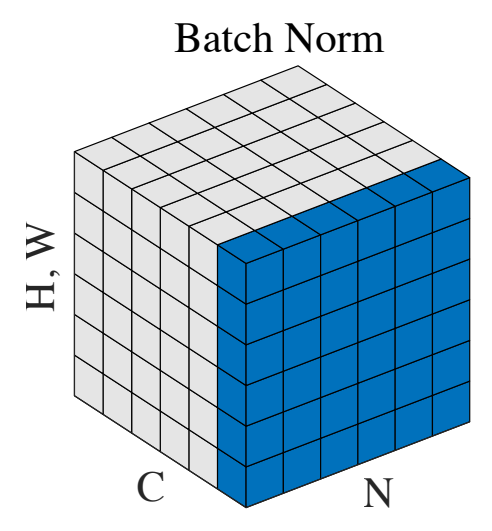
\includegraphics[width=0.3\textwidth]{Images/batch normalization for cnn.png}
	\caption{Batch normalization in CNNs \href{https://arxiv.org/pdf/1803.08494.pdf}{Source}.}
	\label{fig:batch normalization for cnn}
\end{figure}

\vspace{-20pt}

\begin{columns}
\begin{column}{0.6 \textwidth}
\begin{itemize}
	\item BN for FCNs: $\pmb{x}, \pmb{y}: N\times D $
	\item BN for CNNs: $\pmb{x}, \pmb{y}: N\times C \times H \times W $
	\item In both cases: $\pmb{y} = \pmb{\gamma} (\pmb{x} - \pmb{\mu}) / \sqrt{\pmb{\sigma}^2 + \epsilon} + \pmb{\beta}$
\end{itemize}
\end{column}
\begin{column}{0.4 \textwidth}
\begin{itemize}
\item[] $\rightarrow \pmb{\mu}, \pmb{\sigma}, \pmb{\gamma}, \pmb{\beta}: 1\times D$
\item [] $\rightarrow \pmb{\mu}, \pmb{\sigma}, \pmb{\gamma}, \pmb{\beta}: 1\times C \times 1 \times 1$
\item []
\end{itemize}
\end{column}
\end{columns}
\end{itemize}

\end{frame}



